\section{MRI in self-gravitating disks}\label{result1}
In this section we focus on the MRI and use the vertical field setup
of case 1. We first consider MRI modes with negligble density/potential
perturbations to see the effect of self-gravity on the MRI through the
background stratification, then go on to examine MRI modes with
density/potential perturbations in massive disks.  

\subsection{Influence of self-gravity on the MRI through the
  background equilibrium}
Here we use polytropic disks, which have a well-defined disk
thickness. The upper disk boundary is set to $Z_s=0.99H$. We fix
$\beta=100$ and $k_xH=0.1$ unless otherwise stated. 

\subsubsection{Uniform
  resistivity}   
Fig. \ref{compare_growth_poly_uniresis} plots MRI growth rates as a
function of $Q$ and $\Lambda_0$. The resistivity is uniform ($A=1$). 
For ideal MHD ($\Lambda_0>1$), there is negligible dependence on
$Q$. In the resistive limit   
($\Lambda_0<1$), however, growth rates decrease noticeably for $Q<0.5$
($Q_\mathrm{2D}\lesssim 1.5$).  Since we find density and potential
perturbations to be negligible (i.e. the linear response is
non-self-gravitating), this shows that disk self-gravity can affect the
MRI through the background equilibrium.

\begin{figure}
  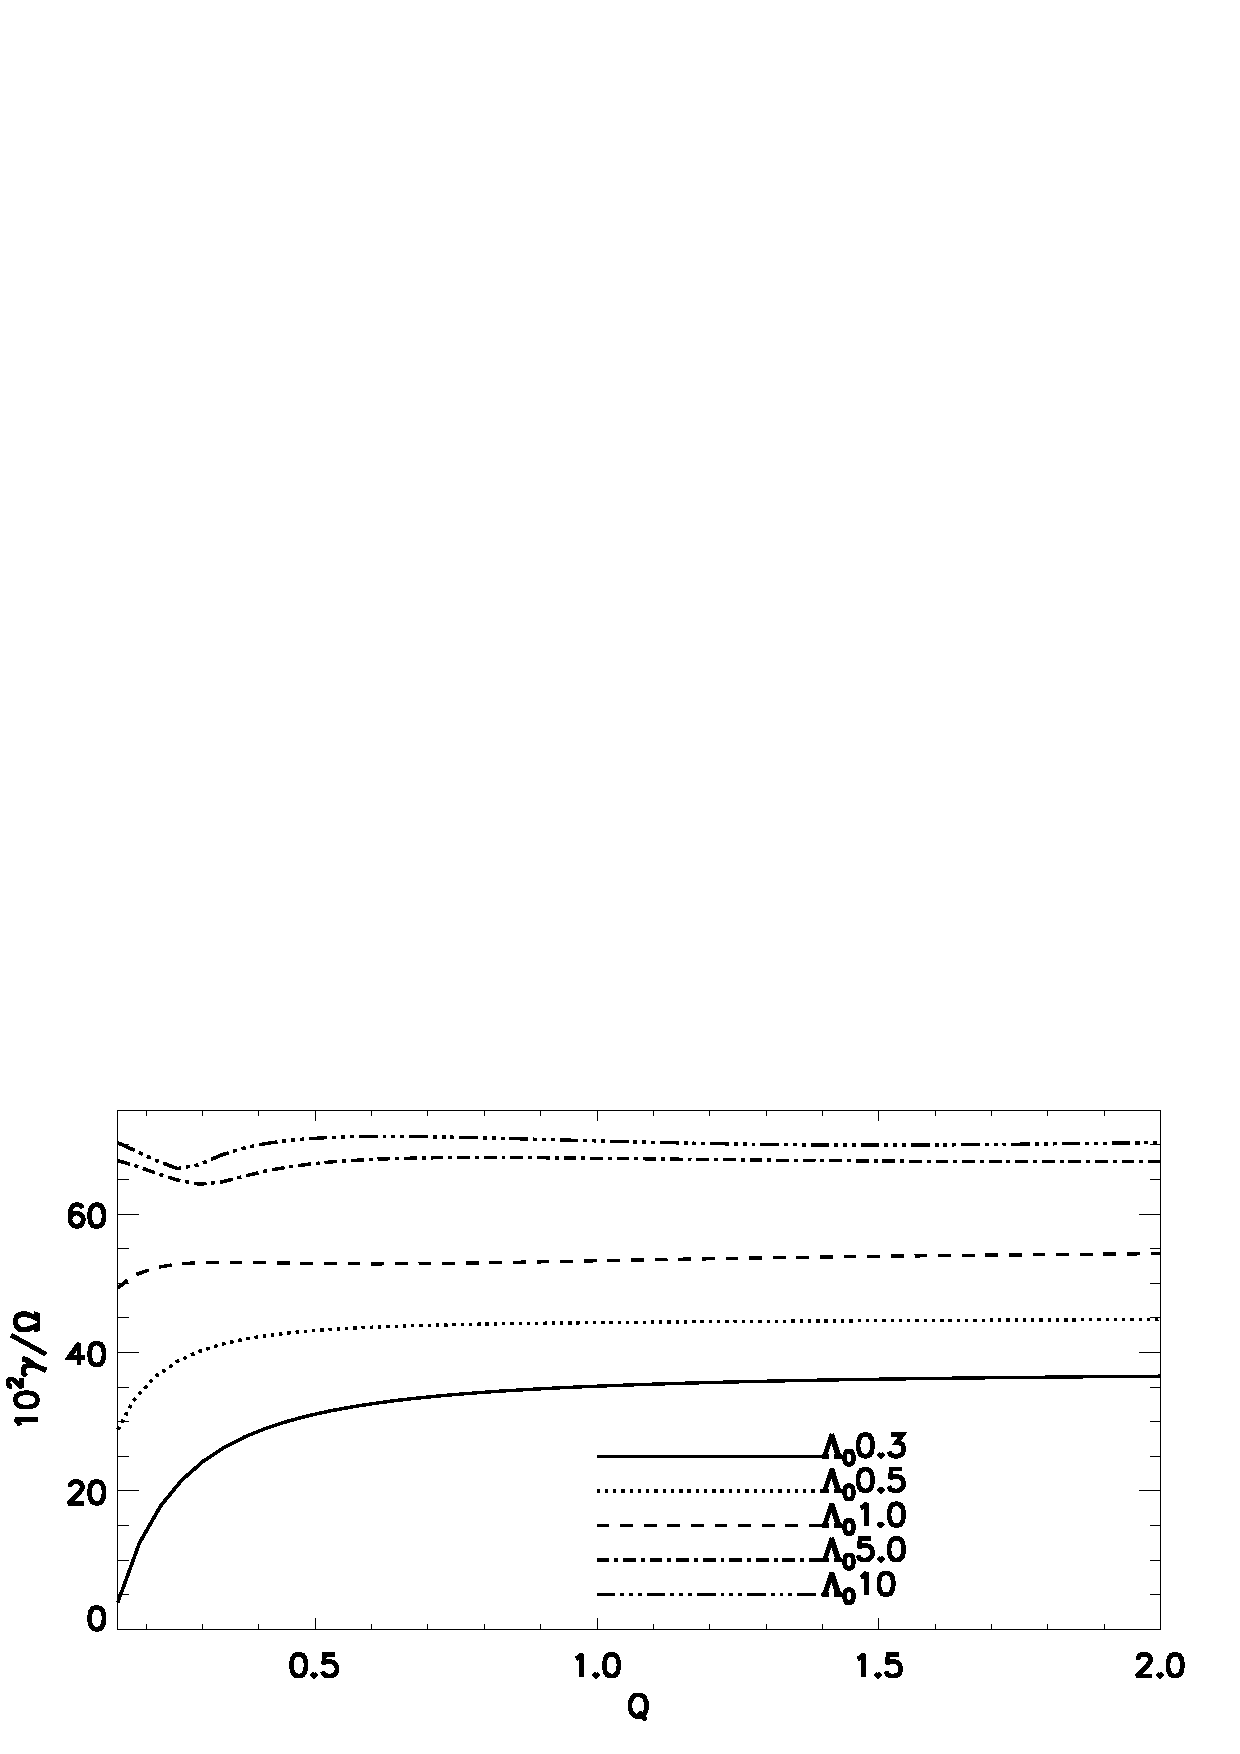
\includegraphics[width=\linewidth]{figures/compare_growth_poly_uniresis2}
  \caption{MRI growth rates as a function of $Q$ and midplane 
    Elsasser numbers, in polytropic disks with $\beta=100$ and uniform
    resistivity.  
    \label{compare_growth_poly_uniresis}}
\end{figure}

\cite{sano99} found that for MRI to operate, its 
wavelength $\lambda$ should fit inside the disk. That is,   
\begin{align}\label{sano_crit}
  \lambda \equiv
  \mathrm{max}\left(\lambda_\mathrm{ideal},\lambda_\mathrm{resis}\right)\lesssim
  2H, 
\end{align}
where the MRI wavelengths are given by 
\begin{align}\label{lambda_ideal}
  \frac{\lambda_\mathrm{ideal}}{2H} = \frac{4\pi}{\sqrt{15}} f \hat{v}_A =
  \frac{4\pi f}{\sqrt{15\beta\hat{\rho}}}
\end{align}
for ideal MHD, and 
\begin{align}\label{lambda_resis}
  \frac{\lambda_\mathrm{resis}}{2H} = \frac{2\pi}{\sqrt{3}}\frac{\hat{\eta}}{\hat{v}_A f} =
  \frac{2\pi f}{\Lambda_0}\sqrt{\frac{\hat{\rho}}{3\beta}} 
\end{align}
in the limit of high resistivity.  
   
Because $\hat{\rho}$ is weakly dependent
on $Q$ (Fig. \ref{eqm_den}), self-gravity only affects the
MRI through the factor $f$, which increases with decreasing $Q$ (see
Fig. \ref{plot_fq} in Appendix \ref{appen1}).   
This implies that sufficiently strong self-gravity can stabilize the
MRI by making $ 2H<\lambda $.   
 
In the ideal limit, we find $\lambda < 2H$ throughout most of the disk
for the values of $Q$ considered, so self-gravity does not affect
growth rates significantly. However, the ratio $\lambda/2H$ does
increase with stronger self-gravity. Consequently, the wavelength of
the instability, in units of $H$, increases. This is shown in
Fig. \ref{compare_result_lambda10} which plots the magnetic energies
for $\Lambda_0=10$ and a range of $Q$ values. The number of vertical
nodes decrease with $Q$, i.e. the disk accommodates fewer wavelengths
because increasing vertical self-gravity makes it thinner. 

\begin{figure}
  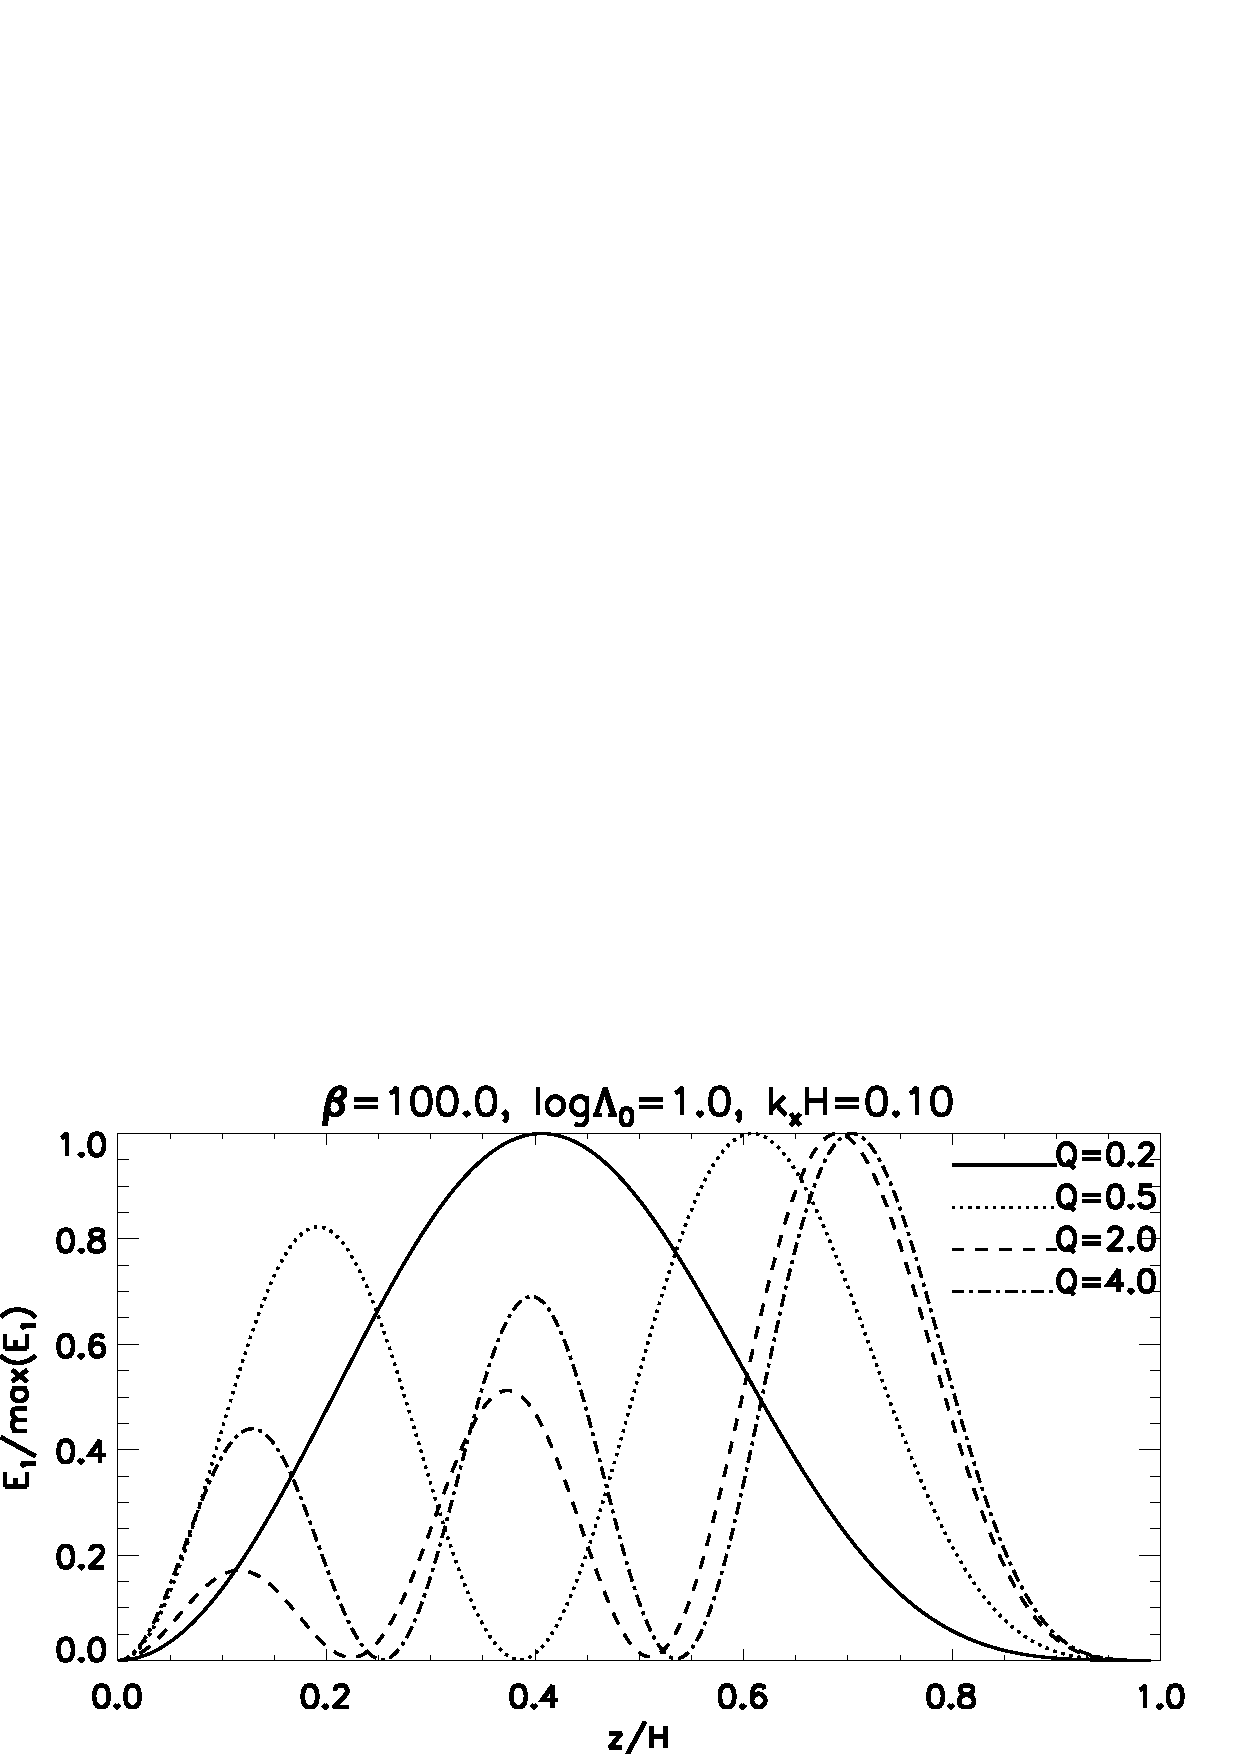
\includegraphics[width=\linewidth]{figures/compare_result_lambda10}
  \caption{MRI magnetic energies in ideal polytropic disks
    for different strengths of self-gravity.    
    \label{compare_result_lambda10}}
\end{figure}


Self-gravity appreciably decreases the MRI growth rates in the
resistive limit. Fig. \ref{lambda_poly_resis} plots 
Eq. \ref{sano_crit} for $\Lambda_0=0.3$. In the non-self-gravitating
disk ($Q=4$) the instability criterion is marginally satisfied and the
MRI operates. As $Q$ decreases, 
Eq. \ref{sano_crit} is violated and the MRI growth rate is
significantly reduced. This is seen for $Q=0.2$ where $\lambda \geq 2H$ throughout
the disk. (The instability is not surpressed since
Eq. \ref{lambda_ideal}---\ref{lambda_resis} is only exact for
unstratified disks.) Although the function 
$f(Q)$ does not change significantly for the range of $Q$ considered,
the dependence of $\lambda_\mathrm{resis}$ on $f(Q)$ is amplified by the
denominator $\Lambda_0<1$ in the resistive case. Modes in
Fig. \ref{lambda_poly_resis} have no nodes in the magnetic energy
$E_m$ except at $z\simeq0,\,H$, i.e. only the longest wavelength survives
with large resistivity. 
%self-gravity tips it over    

\begin{figure}
  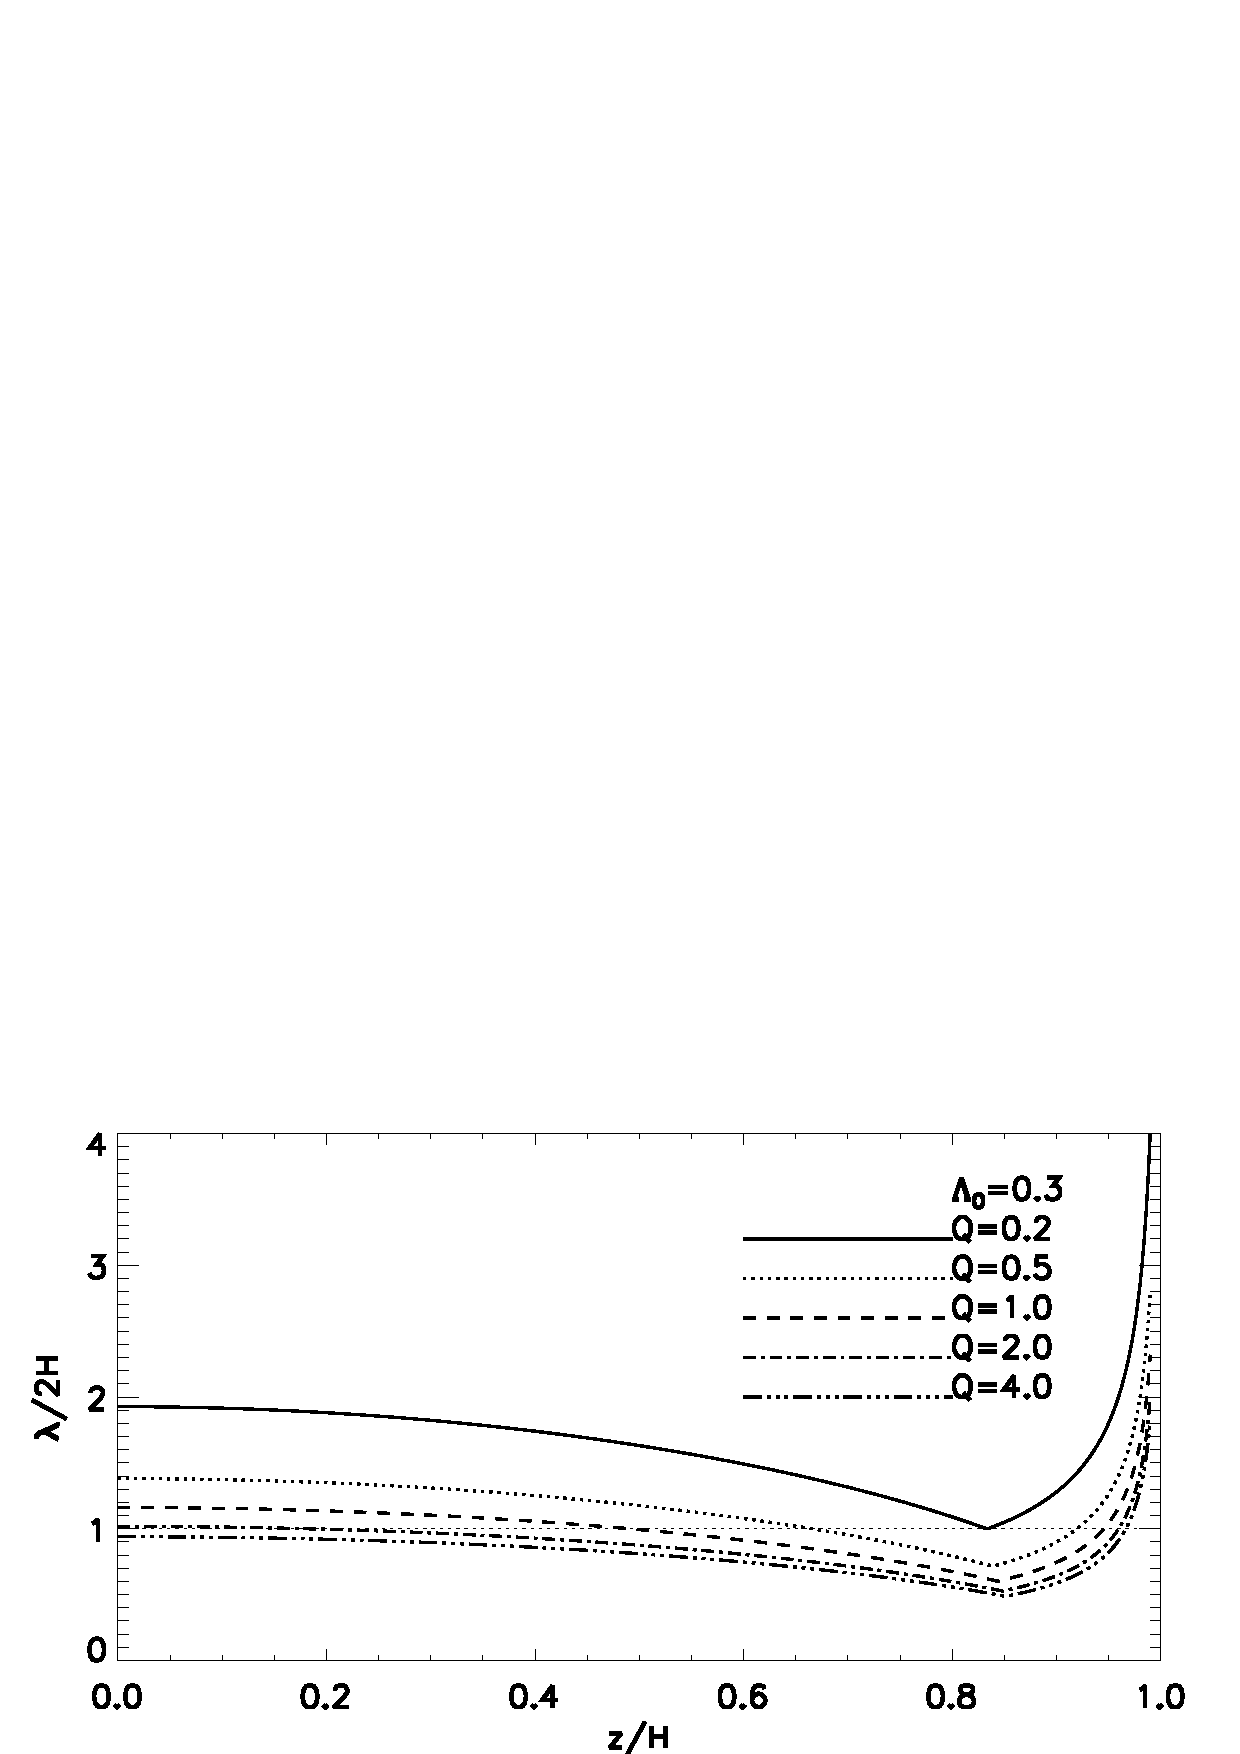
\includegraphics[width=\linewidth]{figures/lambda_poly_uniresis}
  \caption{Approximate wavelengths of the most unstable MRI modes as given by
    Eq. \ref{sano_crit}---\ref{lambda_resis}, normalized by the 
    disk thickness, as a function of height. MRI is expected to
    operate if $\lambda/2H\lesssim 1$. 
    \label{lambda_poly_resis}}
\end{figure}



\subsubsection{Layered 
  resistivity} 
Here we consider disks with midplane Elsasser number $\Lambda_0=0.1$
and a variable resistivity profile with
$A=10^2$. Fig. \ref{poly_layer} compares the magnetic  
energies for $Q=0.2,\,1$ and $4$. They have similar growth rates, $\gamma/\Omega
= 0.53,\,0.64$ and $0.66$, respectively. In the non-self-gravitating
limit ($Q=4$), the MRI is effectively surpressed for
$z\lesssim0.5H$. This is consistent with the picture of layered
accretion proposed for non-self-gravitating disks \citep{gammie96,fleming03}. 
However,in the massive disk ($Q=0.2$) the mode occupies a wider vertical
extent because its wavelength (in units of $H$) is larger. This
suggests that in massive disks, the MRI is not well localized to a
sub-layer within the height, even when the resisitvity has a layered
structure.  


\begin{figure}
  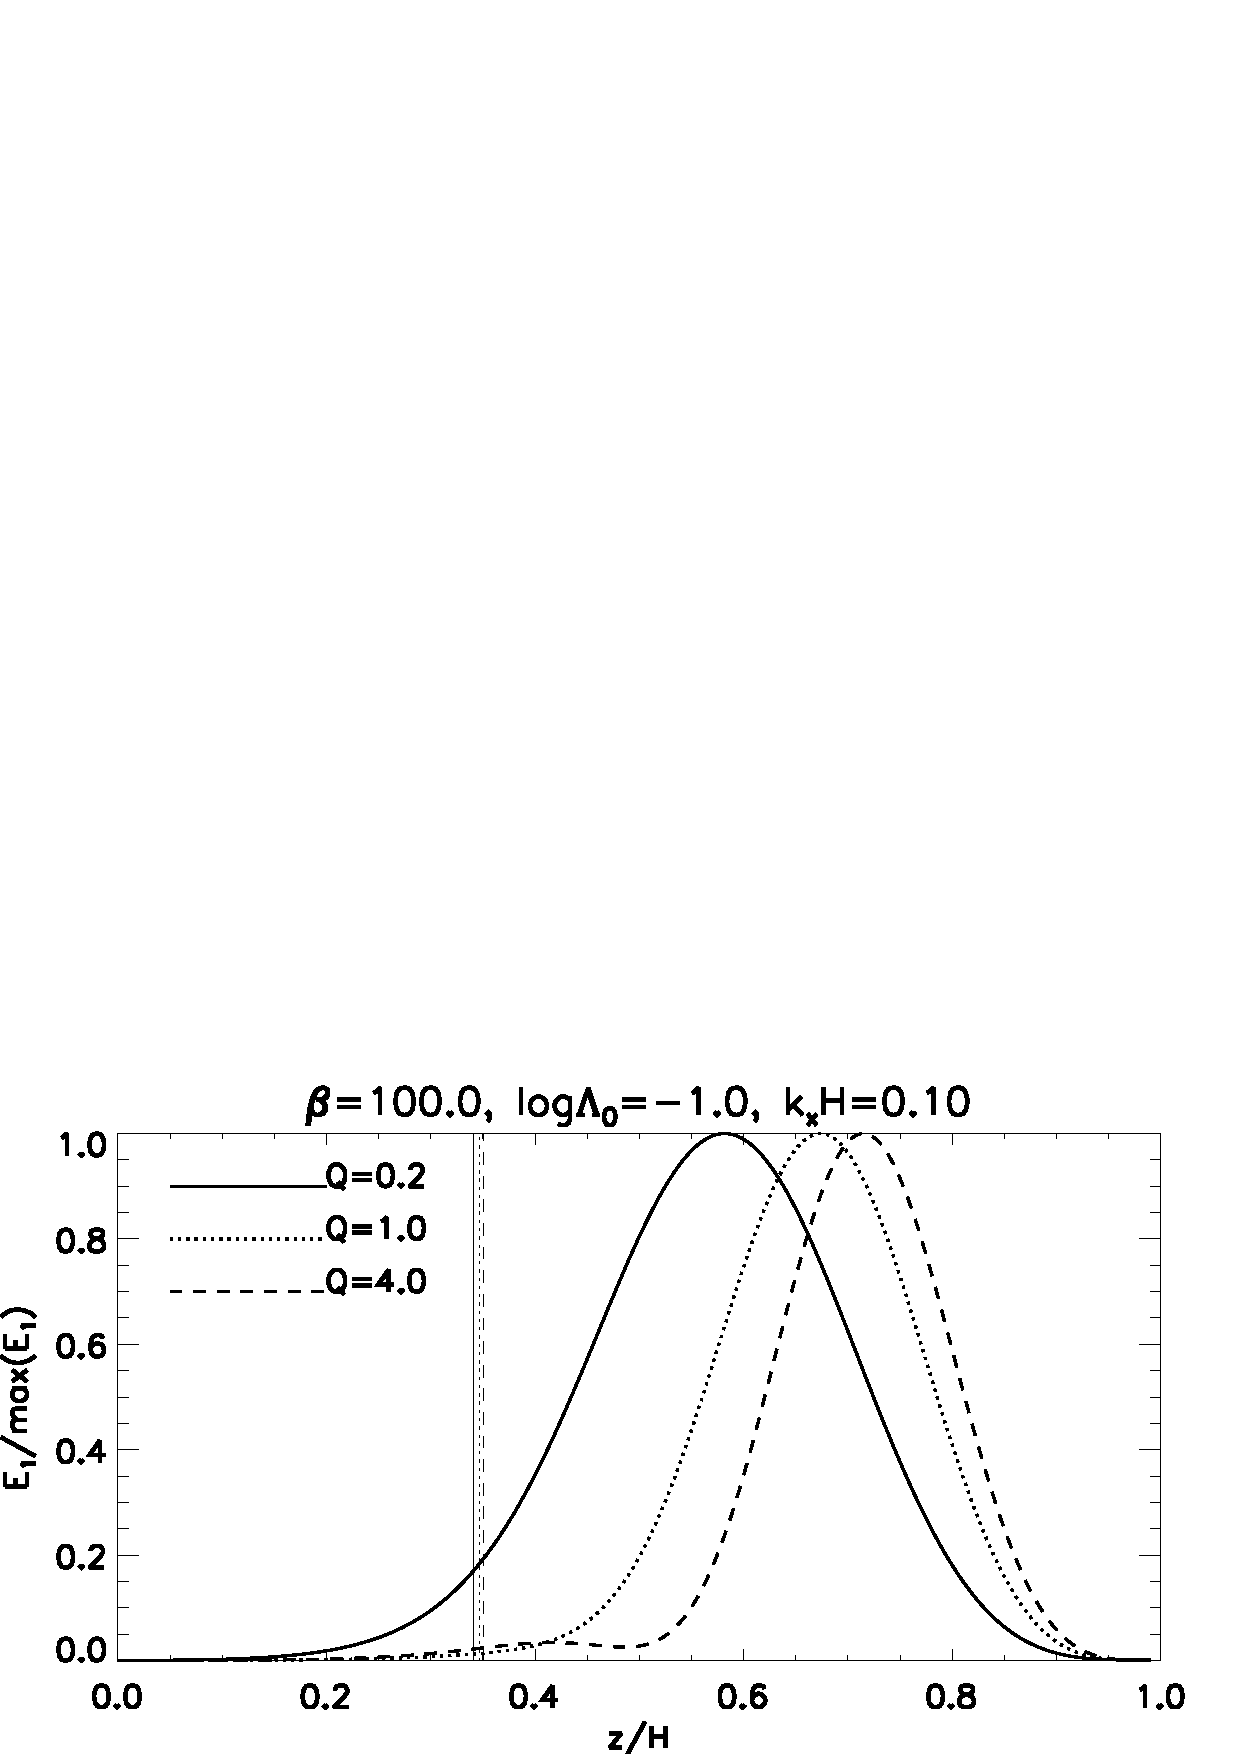
\includegraphics[width=\linewidth]{figures/compare_results_poly_layer_amp100}
  \caption{Magnetic energies as a function of height, for polytropic disks
    in which the conductivity increases by a
    factor $A=10^2$ in going from the midplane to the upper disk
    boundary. The vertical lines indicate $\Lambda=1$ for each value 
    of $Q$.
    \label{poly_layer}}
\end{figure}

\subsubsection{Dependence on $k_x$}
The above experiments show that with increasing 
disk self-gravity, the MRI becomes more global in the vertical
direction. We find a similar result in the horizontal direction. 
Fig. \ref{compare_growth_poly_kx} show MRI growth rates as a
function of $k_x$ for a range of $Q$ values. Increasing self-gravity
decreases the cut-off radial wavenumber for the MRI. We checked
that these modes have negligible density perturbations. Then we can 
understand this result by invoking the instability criteria for  
incompressible MRI in an unstratified Keplerian disk,
\begin{align}
  v_A^2(k_z^2 + k_x^2) < 3\Omega^2,
\end{align}
where $k_z$ is a vertical wavenumber \citep{kim00}. Setting $k_z^2\sim
\Omega^2/v_A^2$ and non-dimensionalizing, we find
\begin{align} 
  k_xH \lesssim \frac{\sqrt{\beta}}{f},
\end{align}
where order-unity factors have been dropped. Despite a simplistic
approach, this demonstrates that with increasing self-gravity
(increasing $f$), we expect MRI modes with small radial
lengthscales to be suppressed.   


 
\begin{figure}
  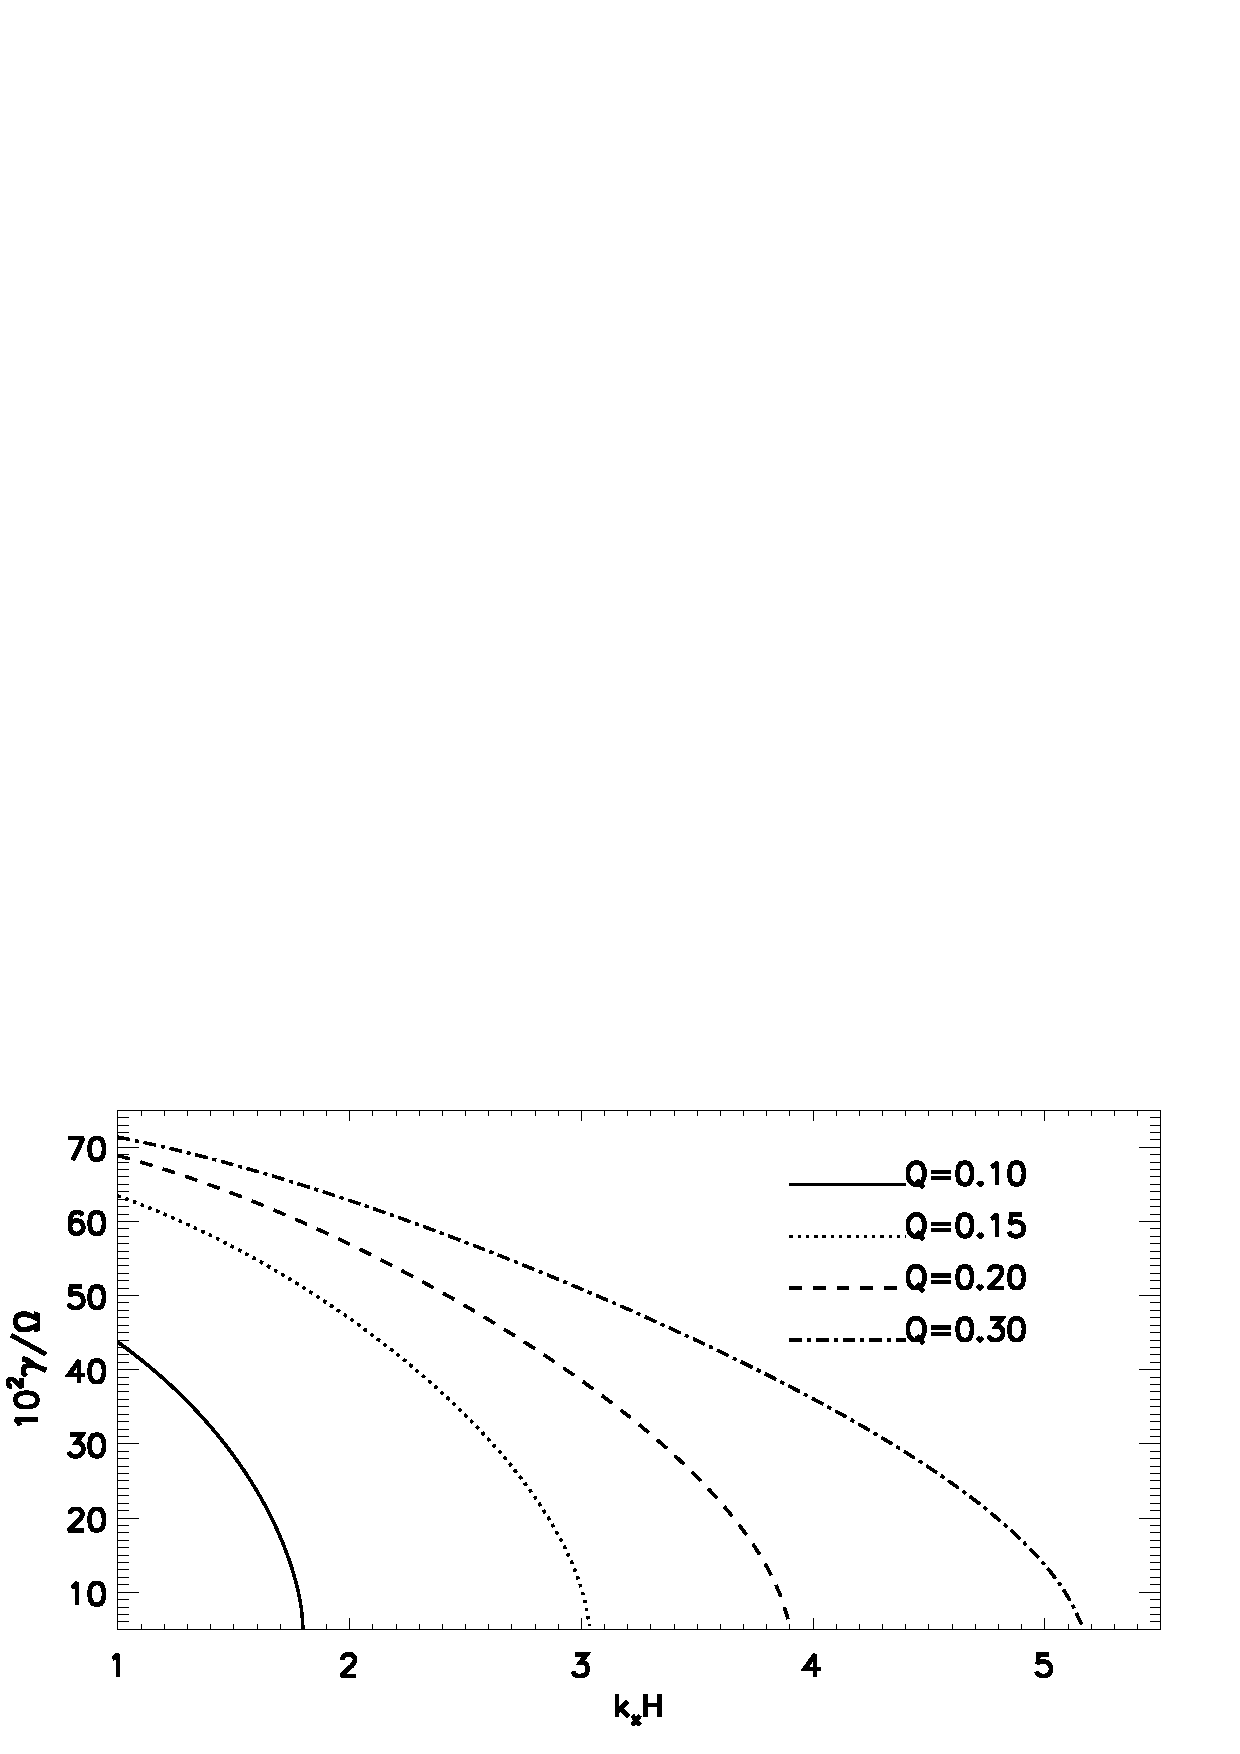
\includegraphics[width=\linewidth]{figures/compare_growth_poly_varQ_kx}
  \caption{MRI growth rates in self-gravitating polytropic disks, as a
    function of the horizontal wavenumber $k_x$. The disk is ideal
    ($\Lambda_0=10^2,\, A=1$) with $\beta = 40$. These modes have negligible
    density/potential perturbations.  
    \label{compare_growth_poly_kx}}
\end{figure}



\subsection{Influence of self-gravity on the MRI through the linear
  response}  
Our goal here is to examine whether or not self-gravity can amplify
the density perturbations associated with the MRI. We compute unstable modes
in a massive isothermal disk with $Q=0.2$ (corresponding to
$Q_\mathrm{2D}=0.72$), which is still expected to be marginally  
stable to gravitational instability \citep[][who find
a critical value of  $Q\simeq 0.2$]{mamat10}.   
The upper disk boundary is set to $Z_s=H$. 

%resolution Nz=256

\subsubsection{Ideal disks}
We first consider ideal MHD by adopting a uniform 
resistivity with $\Lambda_0=100$. %Non-zero density perturbations
%require $k_x\neq0$ so we consider linear modes as a function of $k_x$.   
Fig. \ref{gravity_energy} plots MRI growth rates as a function of
$k_x$ for several values of $\beta$. The curves are color-coded
according to $\tau$. The potential perturbation is
negligible for all cases when $k_xH\lesssim 0.5$, since the MRI
becomes incompressible as $k_x\to 0$. 

\begin{figure}
  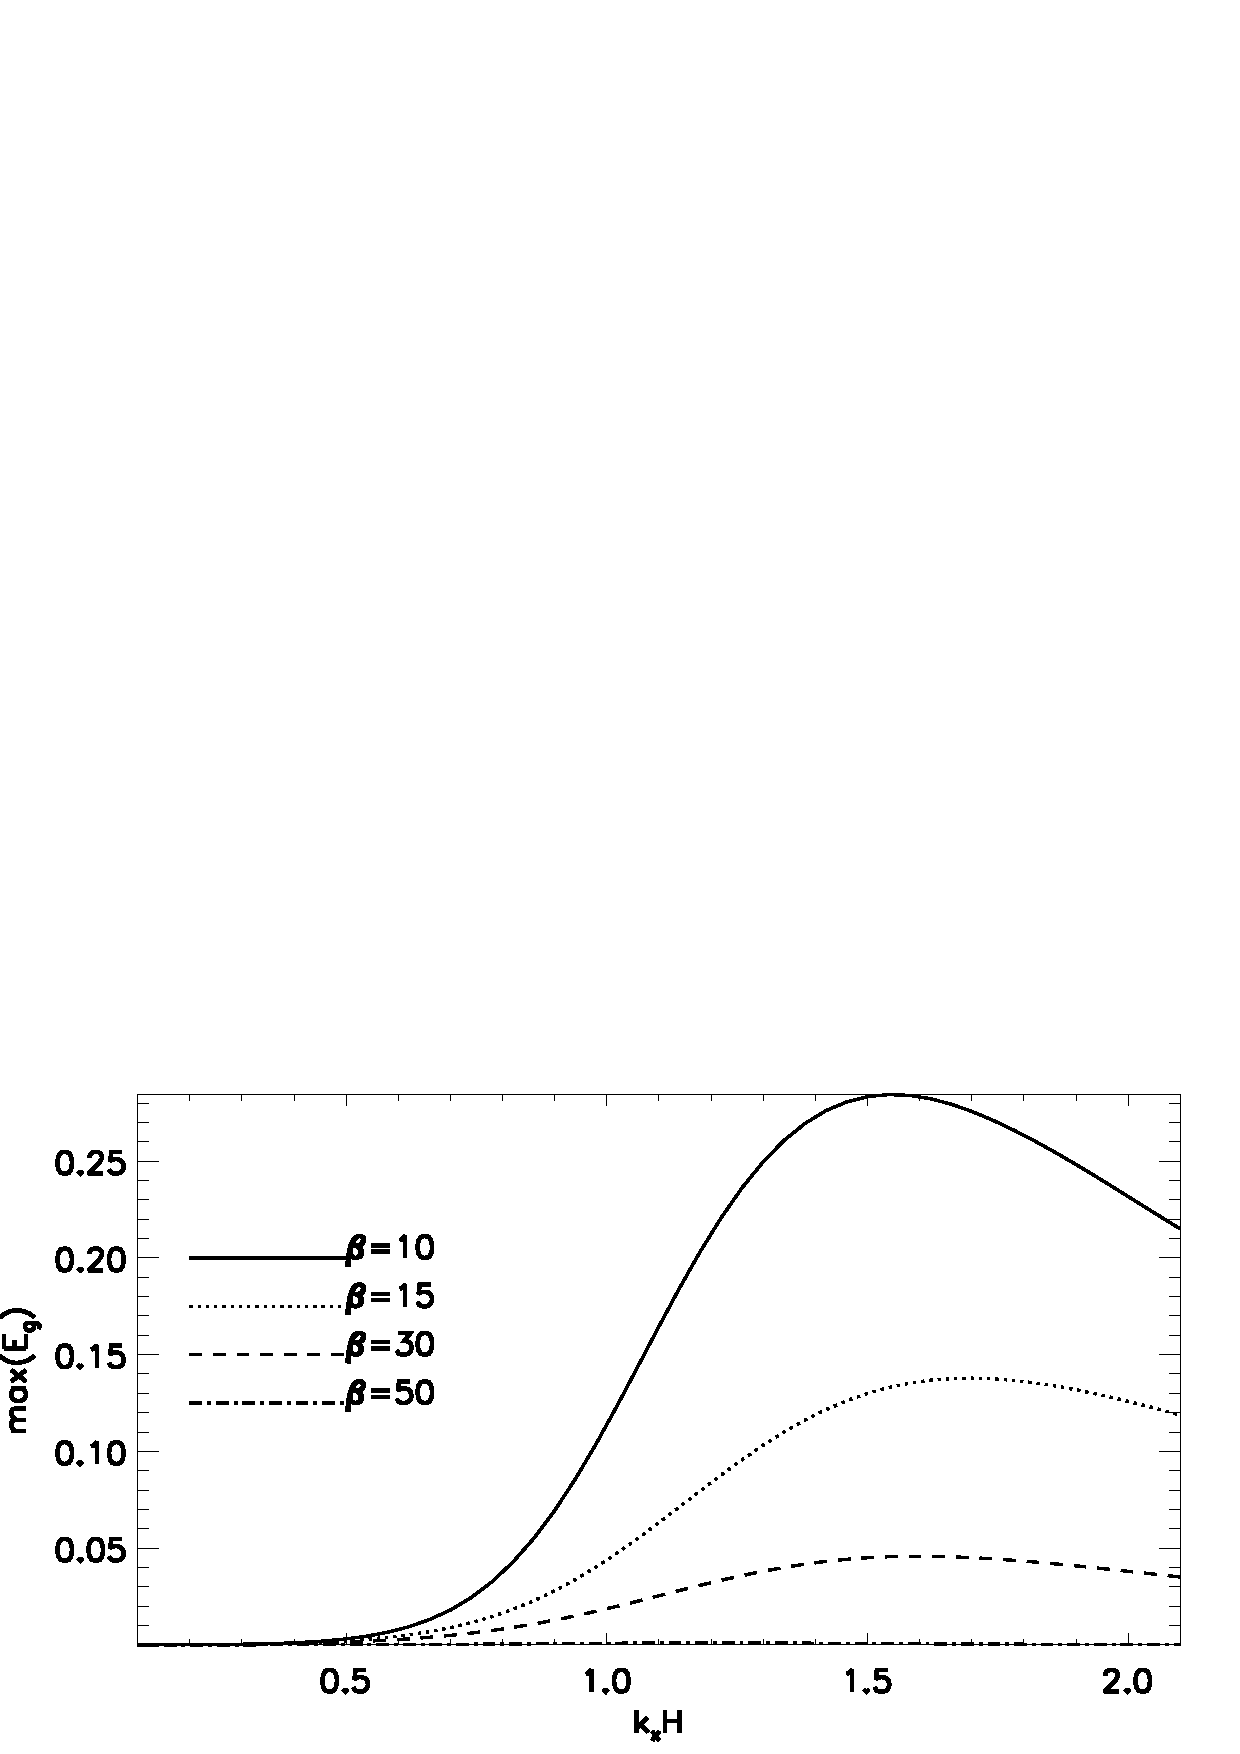
\includegraphics[width=\linewidth]{figures/compare_energy_ideal}
  \caption{Growth rates of MRI modes in an isothermal self-gravitating
    disk with $Q=0.2$ ($Q_\mathrm{2D}=0.72$) in the limit of ideal MHD
    ($\Lambda_0=10^2$), for a range of field strengths $\beta$. The
    colorbar measures the importance of self-gravity by $\tau$.  
    %{\bf ADD BETA=8}
    \label{gravity_energy}}
\end{figure}

For $\beta\gg 1$, i.e. a weak field, density perturbations are
negligible and the standard MRI operates. However, as $\beta$ is
lowered and the MRI growth rate reduced, we find non-negligible
potential perturbation for $k_xH=O(1)$. This suggets that in a
strongly magnetized disk that still permits the MRI, the associated
density perturbation can be important when the disk is
self-gravitating. %but formall stable 


%critical beta, below which MRI is surpressed, increases with the
%strength of self-gravity.

%Fig. \ref{mri_massive} shows an example of a MRI mode with
%non-negligible density perturbation. The growth rate $\gamma\simeq
%0.4\Omega$ is comparable to that of the most unstable mode
%($\gamma\simeq 0.6\Omega$ for $k_x\simeq0$). 
%We therefore expect significant density perturbations to grow
%dynamically, even though the disk is expected to be gravitationally
%stable. 
  
 
%\begin{figure}
%  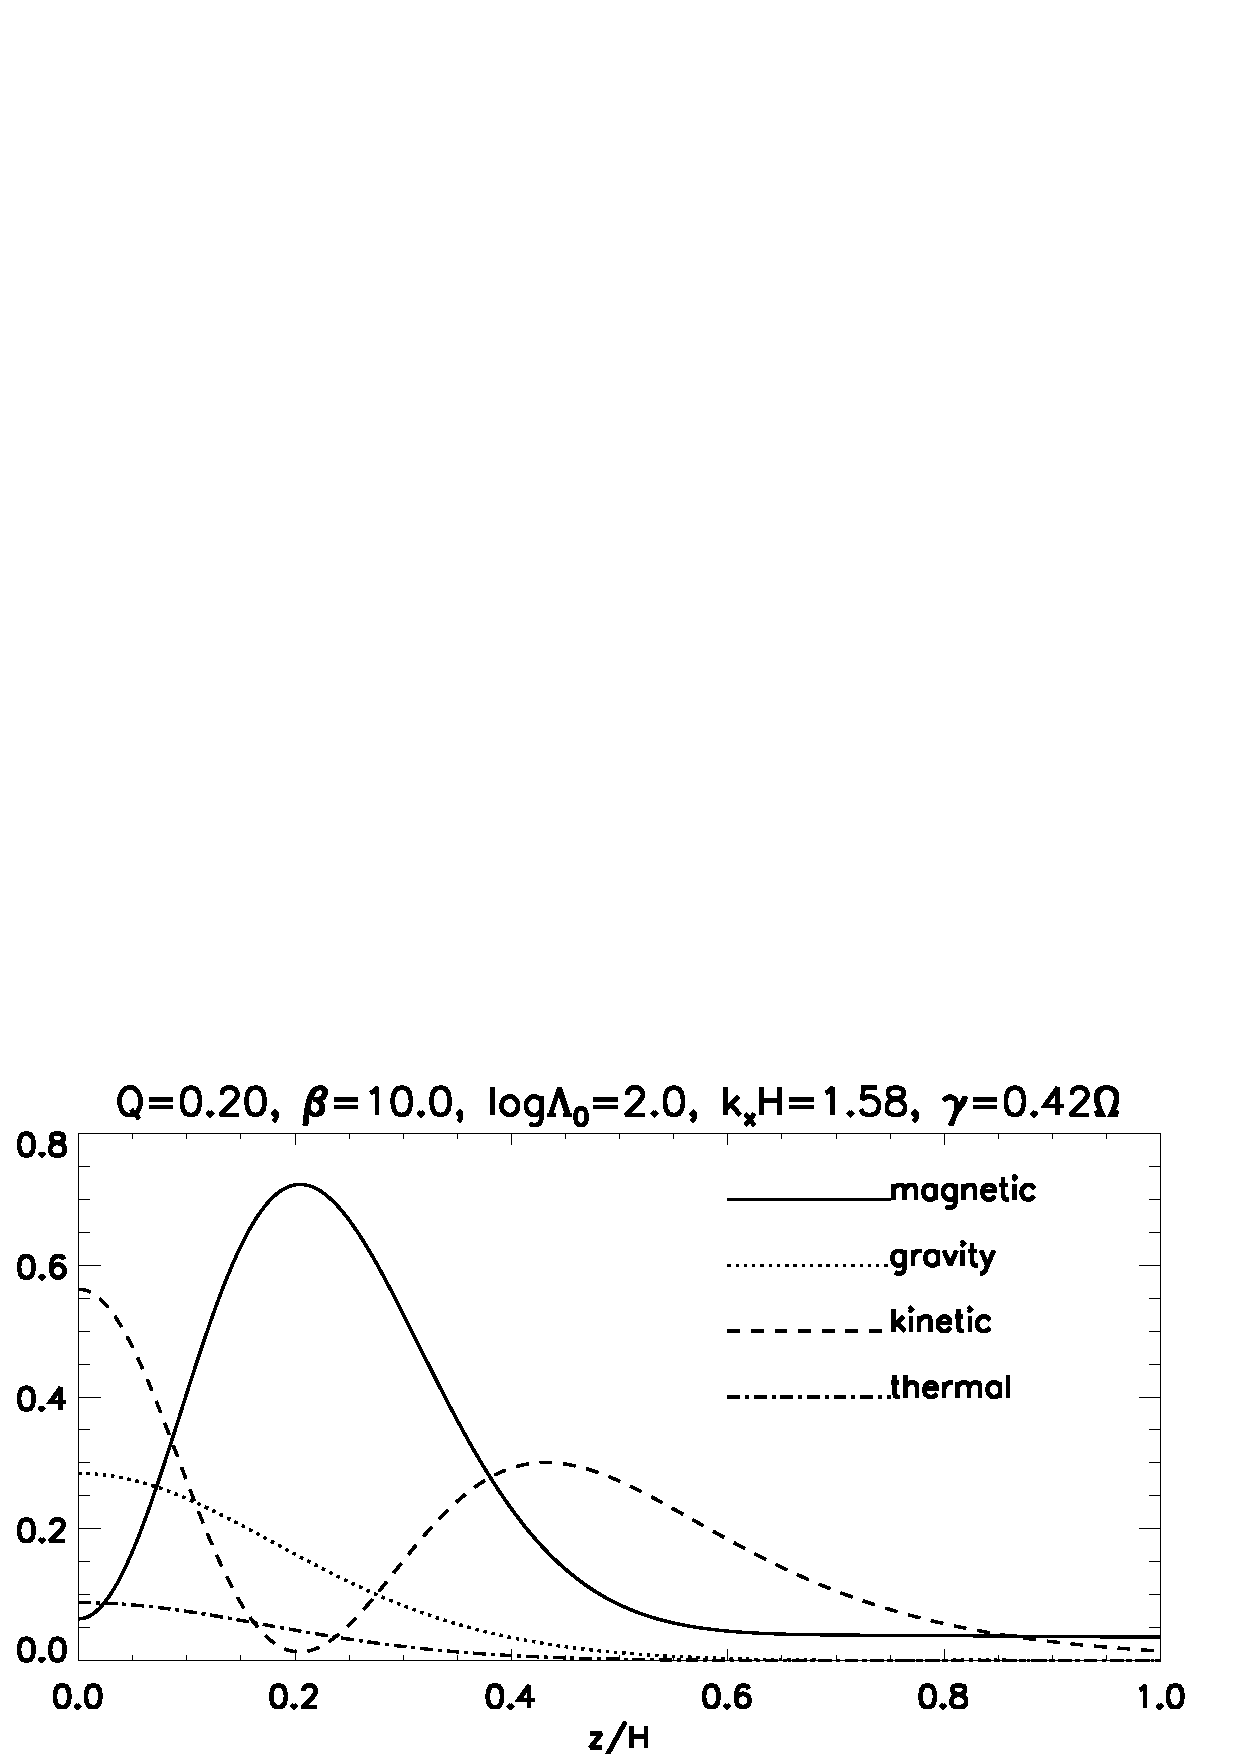
\includegraphics[width=\linewidth]{figures/result_ideal_sg}
%  \caption{Example of a linear MRI mode with non-negligible density and
%    potential perturbation, in a strongly magnetized massive disk
%    ($\beta=10$ and $Q=0.2$) in the limit of ideal MHD 
%    ($\Lambda_0=10^2$).   
%    \label{mri_massive}}
%\end{figure}

\subsubsection{Resistive disks}
We repeat the above calculation for resistive disks, but fix
$\beta=100$ and vary the midplane Elasser number $\Lambda_0$. Growth
rates are shown in Fig. \ref{gravity_energy_resis}. 
Interestingly, in the highly resistive case
the magnetic and gravitational energies can be comparable. For 
$\Lambda_0=0.1$ and $k_xH\simeq1.3$, $\tau\sim 0.3$ which corresponds
to $\avg{E_g}\sim 0.5\avg{E_m}$.  
Fig. \ref{mri_massive_cowling}, we compare the magnetic
energy of this mode to that computed in in the \emph{Cowling  
  approximation}, where the Poisson equation is ignored in the 
linearized equations and the potential perturbation set to zero  
(formally letting $Q\to\infty$ in Eq. \ref{lin_poisson}).  
The growth rate increases slightly when self-gravity is included in the linear
response, since self-gravity is usually destabilizing. However, the
similarity between $\gamma$ and $E_m$ indicates that the instability
in the self-gravitating calculation is fundamentally the MRI.   

\begin{figure}
  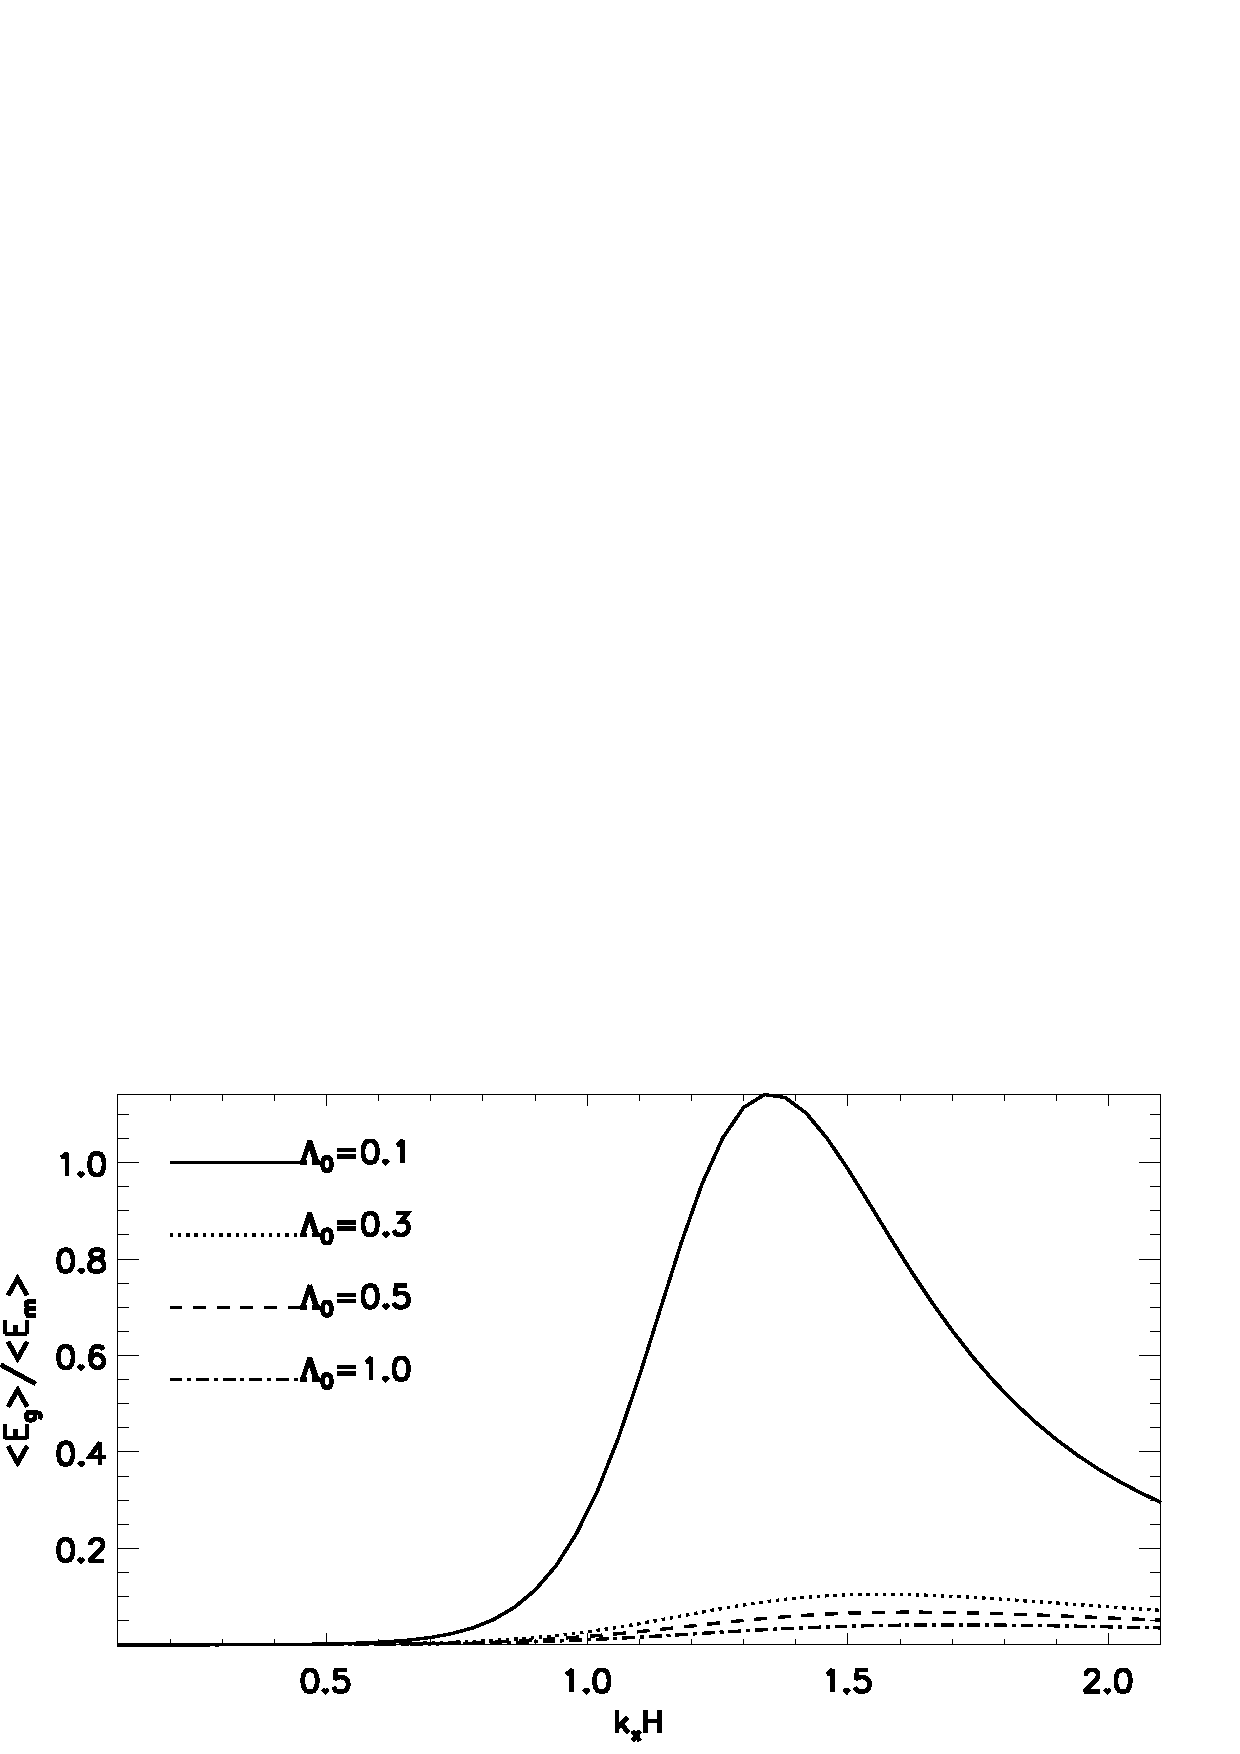
\includegraphics[width=\linewidth]{figures/compare_energy_resis}
  \caption{
    Growth rates of MRI modes in an isothermal self-gravitating
    disk with $Q=0.2$ ($Q_\mathrm{2D}=0.72$) at fixed $\beta=100$, 
    for a range of midplane Elasser numbers. The resistivity is
    uniform. The colorbar measures the importance of self-gravity by $\tau$. 
    \label{gravity_energy_resis}}
\end{figure}


\begin{figure}
  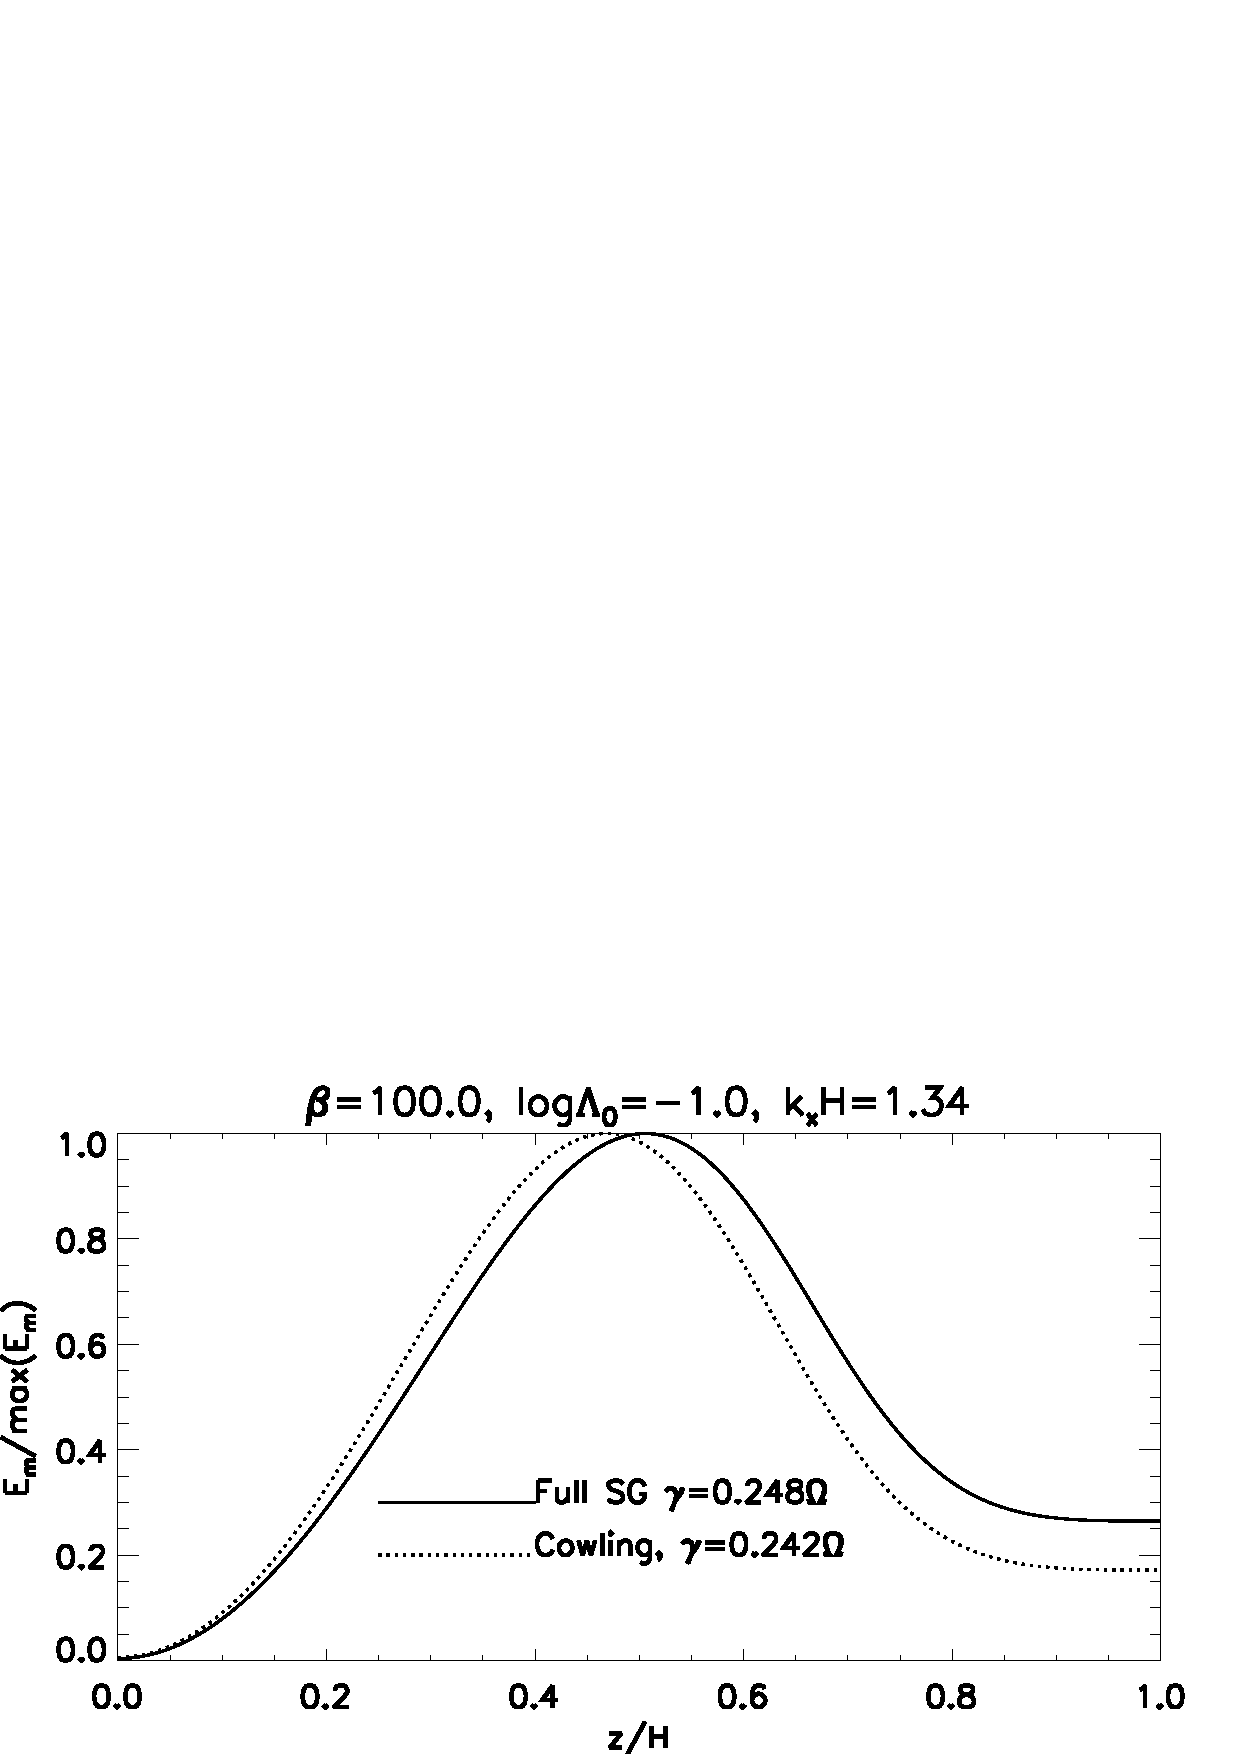
\includegraphics[width=\linewidth]{figures/compare_result_cowling}
  \caption{Magnetic energy associated with the linear mode with
    largest gravitational-to-magnetic energy ratio in
    Fig. \ref{gravity_energy_resis} (solid) compared with that computed
    under the Cowling approximation (dotted). %{\bf REDO FIGURE}
    \label{mri_massive_cowling}}
\end{figure}

Fig. \ref{mri_massive_resis} plots the energies associated with the 
MRI mode discussed above. 
%with $k_xH\sim1.3$ in the $\Lambda_0=0.1$  
%disk. 
The gravitational energy exceeds the 
magnetic energy near the midplane ($z\lesssim0.2H$). The growth rate $\gamma=0.25\Omega$
is not much smaller than that of the most unstable mode
($\gamma=0.36\Omega$ for $k_xH=0.1$), so significant density
perturbations are expected to grow on dynamical timescales for this
system, even though GI should not develop. 

\begin{figure}
  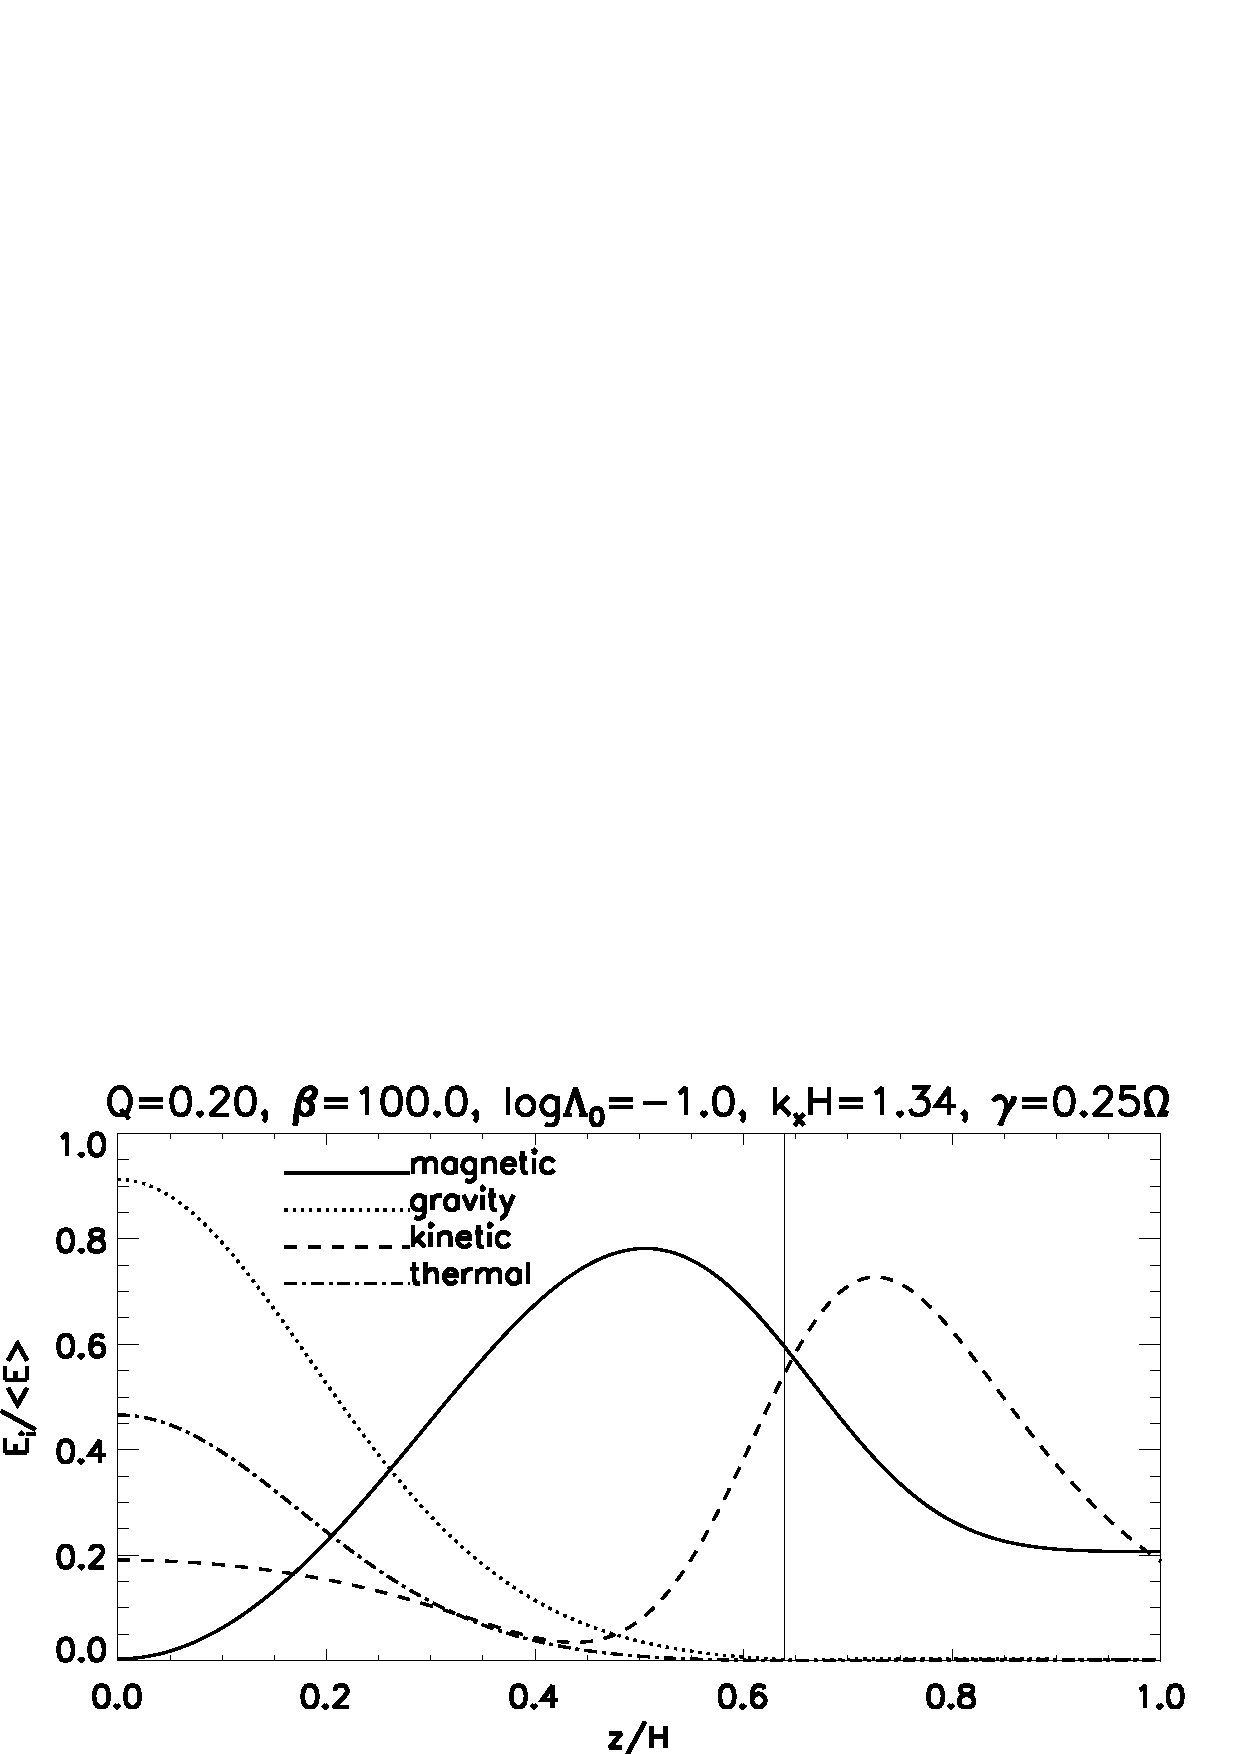
\includegraphics[width=\linewidth]{figures/result_resis_sg}
  \caption{Example of a resistive MRI mode with significant
    gravitational potential perturbation.  The vertical line
    inidicates $\Lambda=1$.  
    \label{mri_massive_resis}}
\end{figure}

\subsubsection{Qualitative interpretation} 
To make sense of the above results, we first return to ideal MHD and 
consider regions close to the disk midplane ($z\sim 0$), where
self-gravity is expected to be most important. For this discussion we
will ignore stratification and set $d^2/dz^2\to -k_z^2$. The governing
equations are then 

\begin{align}
  &  0= v_A^2k^2\dvx + \imgi\sigma\left(\imgi\sigma \dvx - 2\Omega\dvy + \imgi k_x \w\right),\label{simp1}\\
  &  0= v_A^2k_z^2\left(\dvy + \frac{\imgi S
  }{\sigma}\dvx\right) + \imgi\sigma\left(\imgi\sigma\dvy +
  \frac{\kappa^2}{2\Omega}\dvx\right),\label{simp2}\\
  & 0 = -k_z^2\w + \frac{\sigma^2}{c_s^2}W + \sigma k_x \dvx, \label{simp3}\\
  & 0 = k^2\dphi + \frac{\Omega^2}{c_s^2Q}W,\label{simp4}
\end{align}
where $k^2 = k_z^2 + k_x^2$. We imagine an iterative procedure to
solve the above equations, starting from the Cowling approximation. 
%defined to be the
%solution to Eq. \ref{simp1}---\ref{simp3} with potential perturbation
%set to zero. 
This is the standard MRI and we denote the solution as
$\dvx^{(0)}$, $\dvy^{(0)}$ and $W^{(0)}$. 

We now include self-gravity. In general, the compressible MRI has
$W^{(0)}\neq0$. The Poisson equation implies
an associated potential perturbation,    
\begin{align} 
  \dphi = -\frac{\Omega^2}{c_s^2 Q k^2} W^{(0)}.
\end{align}
Physically, we expect $k^2\geq0$, so that a local positive (negative) density
perturbation causes a negative (positive) local potential
perturbation. We then insert $\dphi$ back into the momentum and
continuity equations, and ask how does this potential perturbation
modify the Cowling solution? Writing $\dvx^{(0)} \to \dvx^{(0)} +
\dvx^{(1)}$ and similarly for $\dvy $ and $ W$, we find 
%regard $\dphi$ to alter the Cowling solution, so
%that 
%Then 
\begin{align}
  &   k_x\sigma \dphi = v_A^2k^2\dvx^{(1)} + \imgi\sigma\left[\imgi\sigma
  \dvx^{(1)} - 2\Omega\dvy^{(1)} + \imgi k_x W^{(1)}\right], \label{simp_pert1}\\ 
  &  0= v_A^2k_z^2\left[\dvy^{(1)} + \frac{\imgi S
    }{\sigma}\dvx^{(1)}\right] + \imgi\sigma\left[\imgi\sigma\dvy^{(1)} +
  \frac{\kappa^2}{2\Omega}\dvx^{(1)}\right],\label{simp_pert2}\\
  & k_z^2\dphi  = \left(\frac{\sigma^2}{c_s^2}-k_z^2\right)W^{(1)} +
  \sigma k_x \dvx^{(1)}.\label{simp_pert3} 
\end{align}
Now, if the perturbations to the magnetic field remain
unchanged, i.e. the mode remains close to the standard MRI, then
$\dvx^{(1)} \sim 0$ and $\dvy^{(1)}\sim0$, so Eq. \ref{simp_pert2} is
satisfied. Eq. \ref{simp_pert1} then require $\dphi +
W^{(1)}\sim0$. This is compatible with Eq. \ref{simp_pert3} if 
\begin{align}
  \left|k_z^2\right| \gg \left|\frac{\sigma^2}{c_s^2}\right|. \label{cond}
\end{align}
For the ideal MRI,  we assume $k_z\sim \Omega/v_A$. Then
$|\sigma^2/c_s^2k_z^2|\sim |\sigma^2/\Omega^2\beta|\ll1$ because
$|\sigma|\lesssim \Omega$ and we are considering $\beta\gtrsim 10$. 
Thus Eq. \ref{cond} is generally satisfied.   

The above assumptions imply
\begin{align}
  W^{(1)} \sim \frac{\Omega^2}{c_s^2 Q k^2} W^{(0)},\label{feedback}
\end{align} 
which indicates a non-zero density perturbation due to the
MRI can be amplified by self-gravity. Now, for $k_xH\sim 1$ we have
$|k_z^2/k_x^2|\sim \beta/f^2\gg1$ because $f=O(1)$ and $\beta\gtrsim10$
for the cases considered above. Then
\begin{align}
  \left|\frac{W^{(1)}}{W^{(0)}}\right| \sim \frac{1}{Q\beta}, 
\end{align}
 suggesting stronger amplification of the density field by 
 self-gravity with increasing field strength (decreasing
 $\beta$). 

% not expect significant potential perturbations 
%Conversely, for strong fields, only a single MRI wavelength occupies
%the fluid column. 

 The above arguments can be adapted to the resistive
 disk. Eq. \ref{simp3}---\ref{simp4} are unchanged, while resistive
 terms appearing in Eq. \ref{simp1}---\ref{simp2} only involve the
 potential perturbation through $\w$. For the resistive MRI we assume
 $k_z\sim v_A/\eta$ and $|\sigma|\sim v_A^2/\eta = \Lambda\Omega$
 \citep{sano99}. Then $|\sigma^2/c_s^2k_z^2|\sim 1/\beta \ll 1$ so
 Eq. \ref{cond} is satisfied. Noting that $k_z^2\sim
 \Lambda^2\Omega^2\beta/c_s^2$, the feedback equation becomes
 \begin{align}
   \left|\frac{W^{(1)}}{W^{(0)}}\right| \sim
   \frac{1}{Q\left(f^2\hat{k}_x^2 + \beta\Lambda^2\right)},
 \end{align}
 so increasing the resistivity (decreasing $\Lambda$) should enhance
 density perturbations.  

 %mass contained in small wavelength is small

 For weak fields in an ideal disk, the MRI has a small vertical
 wavelength, $\lambda \ll H$. The perturbed mass contained within
 $\sim \lambda$ is small and its potential
 perturbation is unimportant. Furthermore, considering the stratified
 disk, $\lambda\ll H$ imply rapid variations in the density
 perturbation across the disk height, averaging to zero, so the
 magnitude of the associated potential perturbation is small. 
% because the gravitational potential is the integral of the density
% field, i
 Self-gravity does not affect the MRI in this regime.   
 
 %, i.e. internal cancellations would occur when such an integral is
 % performed.   
 
 However, a strong field and/or large resistivity increases the MRI
 vertical wavelength. When the vertical scale of the MRI becomes
 comparable to the disk thickness, i.e. $\lambda\sim H$, the
 perturbed mass across the disk height can contribute to a net potential
 perturbation. We therefore expect self-gravity to be important for
 the MRI when it is weak.  

%The perturbed mass
% within the unstable mode corresponds to that in the within 
%This can give rise to a net
% potential perturbation  
 %Self-gravity can then be effective, since it
 % operates globally in the vertical direction. 
%GI of 3D disks can be
 %analysed in vertically-integrated
 %systems 
%coupling to SG 
%That is when the MRI is weak
